\documentclass[hyp]{socreport}

\usepackage{fullpage}
\usepackage{url}
\usepackage{amsmath}
\usepackage{amsfonts}
\usepackage{graphicx}
\usepackage{pgf}
\usepackage{tikz}
\usepackage[latin1]{inputenc}
\usepackage{verbatim}
\usetikzlibrary{fit}					% fitting shapes to coordinates
\usetikzlibrary{backgrounds}	% drawing the background after the foreground
\usetikzlibrary{arrows,automata,calc,patterns,snakes}

\begin{document}
\pagenumbering{roman}
\title{Predicting Web 2.0 Thread Updates}
\author{Shawn Tan}
\projyear{2012}
\projnumber{H079830}
\advisor{A/P Kan Min-Yen}
\deliverables{
	\item Report: 1 Volume
}
\maketitle
\begin{abstract}
In this report, we study a problem and design an efficient algorithm
to solve the problem.  We implemented the algorithm and evaluated
its performance againts previous proposed algorithms that solves the
same problem.  Our results show that our algorithm runs faster.

%TODO
\begin{descriptors}
    \item C5 Computer System Implementation
	\item G2.2 Graph Algorithms
\end{descriptors}
\begin{keywords}
	Problem, algorithm, implementation
\end{keywords}
\begin{implement}
	python, bash
\end{implement}
\end{abstract}

\begin{acknowledgement}
\end{acknowledgement}

\listoffigures 
\listoftables
\tableofcontents 

\chapter{Introduction}
	With the advent of Web 2.0, sites with forums, or similar thread-based
discussion features are increasingly common.  Our goal in this thesis
is to create an algorithm that can predict when updates in such
threads will occur.
\begin{table}\label{table:web20}
	\makebox[\textwidth][c]{
	{\footnotesize
	\begin{tabular}{|l|c|c|c|c|c|c|c|c|c|c|}
		\hline
			\input{tables/web20}
		\hline
	\end{tabular}
	~\\
	}
	}
	{\footnotesize
\caption{Features of popular Web 2.0 sites}
	\begin{tabular}{l l}
		T &= Twitter mentions\\
	 FB L &= Facebook Likes \\
		FB S &= Facebook Shares\\
	G +1 &= Google +1\\
		   L&= Likes (Local) \\
   		DL &= Dislikes (Local) \\
			C &= Comments \\
		PV &= Page Views \\
   Follows &= Site-local feature for keeping track of user's activities
	\end{tabular}
}
\end{table}

Table \ref{table:web20} shows us that many of the popular Web 2.0
sites have comment features. This suggests that content on the web is
increasingly being created by users alongside content providers.

%we are predicting web 2.0 updates
In an increasing number of cases, news travels more quickly through
online community discussions than through traditional media. Users also
typically discuss purchased products bought online on forums,
and companies that want to get timely feedback about their product
should turn to data mined from such sites.

Web crawling is largely IO-bound, a large portion of the time spent crawling is 
waiting for the server to supply a response to the request issued by the 
crawler. However, for sites with a large number of pages ( as in popular forum 
sites ), make this infeasible in practice. On top of the usual requests it has, 
it then has to deal with repeated requests from such a crawler. Most sites do 
not mind some additional bandwidth, but if it gets excessive, it may be 
construed as a Denial-of-Service attack. At best, the site may deny any further 
requests from the crawler, and at worst the large number of requests may bring 
down the site.
% bandwidth use but too much is not a good thing.  See white-hat rules
% about spiders.

A simple method to reduce the amount of polling needed is to use the
average time differences between previous posts to estimate the
arrival of the next one, and to abstain from polling until the
estimated time.
% Min: you need to discuss how well this simple baseline does and whether it is 
% actually adopted.

A key observation in our work is that the contents of the thread may
also influence the discussion and hence the rate of commenting.  We
believe that the content of the thread has information that can give a
better estimate of the time interval between the last post and a new
one.

% Min: tie the ``hypothetical'' example with actual posts.  Also, your
% introduction needs to actually carry through to the final
% implementation and experimentation where you use such features to
% estimate properly.
For example, a thread in a technical forum about a Linux distribution may start 
out as a question. Subsequent questions that attempt to either clarify or expand 
on the original question may then be posted, resulting in a quick flurry of 
messages. Eventually, a more technically savvy user of the forum may come up 
with a solution, and the thread may eventually slow down after a series of 
messages thanking the problem solver. 

% Min: your introduction needs some work.
% Towards the end you need.  Please restructure the below.
% 1) a clear problem statement
% 2) statements of the contribution of your work
% 3) A navigation paragraph that describes how the rest of the report
% is going to be structured, especially if it deviates from ``normal''
% structure.
Let us define all such thread-based discussion styled sites as forums. Ideally, 
an incremental crawler of such user-generated content should be able to maintain 
a fresh and complete database of content of the forum that it is monitoring.  
However, doing so with the previously mentioned naive method would (1) incur 
excessive costs when downloading un-updated pages, and (2) raise the possibility 
of the web master blocking the requester's IP address.

Our high level goal: To come up with a suitable algorithm for revisiting user 
discussion threads, based on the discussion content in the thread. In this 
project, we focus on forum threads. We demonstrate three different methods for 
achieving this using regression methods, and also propose a new metric for 
measuring the timeliness of such a model that balances between the model's 
timeliness and bandwidth consumption.



\chapter{Related Work}
	\section{Refresh policies for incremental crawlers}
In order to devise such a strategy, we need to predict how often any user may 
update a page. Some work has been done to try to predict how often page content 
is updated, with the aim of scheduling download times in order to keep a local 
database fresh.


We will discuss the \emph{timeliness} of our crawler to maintain the freshness 
of the local database, which refers to how new the extracted information is. Web 
crawlers can be used to crawl sites for user comments and threads for 
postprocessing later. Web crawlers which maintain the freshness of a database of 
crawled content are known as incremental crawlers. Two trade-offs these crawlers 
face cited by Yang et. al. 2009 \cite{Yang2009} are \emph{completeness} and 
\emph{timeliness}. \emph{Completeness} refers to the extent which the crawler 
fetches all the pages, without missing any pages. \emph{Timeliness} refers to 
the efficiency with which the crawler discovers and downloads newly created 
content. We focus mainly on timeliness in this project, as we believe that 
timely updates of active threads are more important than complete archival of 
all threads in the forum site.

Many such works have used the Poisson distribution to model page updates.  
Coffman et. al. \cite{Coffman1997} analysed the theoretical aspects of doing 
this, showing that if the page change process is governed by a Poisson process 
$\lambda e^{-\lambda \mu}$, then accessing the page at intervals proportional to 
$\mu$ is optimal.

Cho and Garcia-Molina trace the change history of 720,000 web pages collected 
over 4 months, and showed empirically that the Poisson process model closely 
matches the update processes found in web pages\cite{Cho1999}. They then 
proposed different revisiting or refresh policies 
\cite{Cho2003,Garcia-molina2003} that attempt to maintain the freshness of the 
database.

The Poisson distribution were also used in Tan et. al. \cite{Tan2007} and Wolf 
et. al. \cite{Wolf2002}. %elaborate!!!!
However, the Poisson distribution is memoryless, and in experimental results due 
to Brewington and Cybenko \cite{Brian2000}, the behaviour of site updates are 
not. Moreover, these studies were not performed specifically on online threads, 
where the behaviour of page updates may be very different from that of static 
pages.

Yang et. al. \cite{Yang2009}, attempted to resolve this by using the list 
structure of forum sites to infer a sitemap. With this, they reconstruct the 
full thread, and then use a linear-regression model to predict when the next 
update to the thread will arrive. %elaborate!!!

Online forums and bulletins have a logical, hierarchical structure in their 
layout, which typically alerts the user to thread updates by putting threads 
with new replies at the very top of the thread index. Yang's work exploits this 
as well as their linear model to achieve a predicton of when to retrieve the 
pages.
However, this is not so for comments found on blog sites or discussion threads 
in an e-commerce site about a certain product and the lack of these pieces of 
information may result in a poorer estimate, or no estimate at all.


Our perspective is that the available content on the thread at the time of the 
retrieval should also be factored into the model used to predict the page 
updates. Next, we look at some of the related work pertaining to thread content.

\section{Thread content analysis}
While there is little existing work using content to predict page updates, we 
will review some existing work related to analysing thread-based pages which we 
think will aid us in our efforts to do content-based prediction.

Wang et. al \cite{Wang2011} did work in finding out linkages between forum posts 
using lexical chaining. They proposed a method to link posts using the tokens in 
the posts called $Chainer_{SV}$. While they do analyse the content of the 
individual posts, the paper does not make any prediction with regards to newer 
posts. The methods used to produce a numeric similarities between posts may be 
used as a feature to describe a thread in its current state, but incorporating 
this into our model is non-trivial.

%Kleinberg used Hidden Markov Models to predict ``bursts" in message arrival 
%times \cite{Kleinberg2003}. In his running example, he used email messages, and 
%used time between messages to estimate the states that produced the sequence.  
%While the model may be able to predict what the state is for the next time 
%interval, it does so using the history of message arrival times, and does not 
%take into account the content within the messages themselves.


%One also cannot ignore the fact that social factors play a role when users 
%interact in an online discussion. Granovetter's threshold model for social 
%behaviour may also be useful in describing how the users behave as a whole.

With these related work in mind, we next propose our modelling of a thread as a 
Markov chain, and our approach to solving the problem.


\chapter{Method}
	\documentclass[12 pt]{article}
\usepackage{amsmath}
\usepackage{url}
\usepackage{graphicx}
\usepackage{setspace}
\usepackage{pgf}
\usepackage{tikz}
\usetikzlibrary{arrows,automata}
\usepackage[latin1]{inputenc}
\usepackage{verbatim}
\usepackage{lscape}
%\usepackage[margin=1.2in]{geometry}

	\addtolength{\oddsidemargin}{-.5in}
	\addtolength{\evensidemargin}{-.5in}
	\addtolength{\textwidth}{0.75in}
	\addtolength{\topmargin}{-1in}
	\addtolength{\textheight}{1.75in}
\begin{document}

\newcommand{\vocab}{\mathbf{v}}
\newcommand{\dtvec}{\mathbf{t}_\Delta}
\newcommand{\ctxvec}{\mathbf{t}_\text{ctx}}
\newcommand{\dt}{\Delta_t}


\section{Method}

Extract data collected from forums Timestamp, Author, Text Content. Using sliding window training method, group consecutive $w$ posts together and perform regression on $\Delta_t$. More formally, we are trying to learn a function $f$ such that $f(\mathbf{x}_{t-w},\hdots, \mathbf{x}_{t-1}) \approx \Delta_{t}$, where $\mathbf{x}_t$ is a post made at time $t$, and $\Delta_t$ is the time between the $t$-th post and the $(t-1)$-th post. The following are the features used:
\begin{description}
	\item[Previous time differences] All the time differences between posts made in the window. ($\mathbf{t}_\Delta$)
	\item[Time-based features] Day of week, Hour of day. Provides contextual information about when the post was made. ($\mathbf{t}_{\text{ctx}}$)
	
	\item[Content features (text)] Word frequency counts. Used regression to test effect of single regressor. Top $F$ features are selected for extraction. ($\mathbf{w}$)

\end{description}

\subsection{Evaluation metrics}
We use \emph{Mean Absolute Percentage Error} (MAPE), to measure the performance of the learnt model. This value does not reflect how well the model will do in a real-time setting, but gives an idea of how far off the model is given a window. This value is given by
\[
	\frac{1}{N}\sum^N_{i=1}\left|\frac{A_i-F_i}{A_i}\right|
\]

The \emph{$T$-score} metric measures the performance on a thread. This is the average time taken between a post being made and a visit made to retrieve that post. Limitations are that the value $T$-score does not factor in the number of times the page is hit. Keep track of the number of visits made as well. (Include explanation of $T$-score)

Viewing the posts made during the thread's lifetime as segmentations of the thread, and the visits made as hypotheses of where the segmentations are, we use the $Pr_{error}$ metric from Georgescul et. al. , 2006 as a measure of how close the predictions are to the actual posts.





\section{Results}

The results for experiments done with different combinations of the above specified features are shown in Table \ref{expt1}.
\begin{table}
	\footnotesize
	\begin{centering}
	\begin{tabular}{|l|c|c|c|c|c|c|c|c|}
	\hline
	\input{init_res}
	\hline
	\end{tabular}
	\caption{Experiment results}
	\label{expt1}
\end{centering}
\end{table}

Overall average and window average perform very poorly, on MAPE score, reflected in $T$-score.

Looking at $T$-score and no. of visits together, would seem that $\textbf{t}_\Delta$ is important feature (Including reduces $T$-score).

Using content (word frequency) features for prediction, gives only slight improvement.

High values for $Pr_{miss}$ and low for $Pr_{fa}$, are due to

	Mainly due to $Pr_{miss}$ being conditioned on the fact that there must be a segmentation/post there.
	Posts come in bursts, visits are fairly periodic, and intervals between visits are larger than post bursts.
	More posts than visits in places with posts, hence higher $Pr_{miss}$

	High no. of invalid predictions.
\begin{landscape}
\begin{figure}
	\centering
	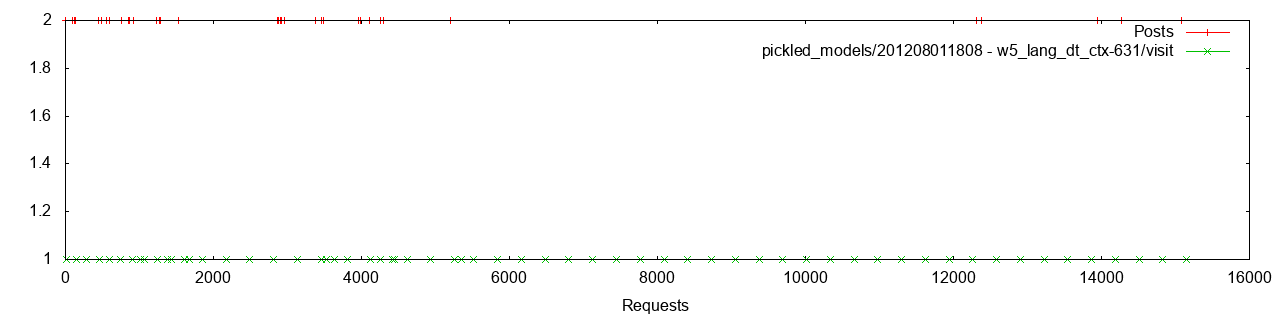
\includegraphics[scale=0.5]{example_seq.png}
	\caption{Visitation chart for a model using the $w=5, \mathbf{t}_\Delta, \mathbf{t}_{\text{ctx}},\mathbf{w}$ feature set. Invalid Predictions = 0.758, $Pr_{error} =  0.485$, $T$-score = 119.612, Posts = 41, Visits = 62}
\end{figure}
\end{landscape}


\bibliographystyle{acm}
\bibliography{report}
\end{document}

\chapter{Evaluation}
	One of the contributions of this project was also to come up with a good metric 
for measuring the performance of a model that performs predictions. Our metric 
has to be different from traditional methods of measuring performance, like Mean 
Average Percentage Error (MAPE), for instance. In such measures, the performance 
of the model is measured on an instance by instance basis. To give a concrete 
example, say we are attempting to predict stock prices. Given the feature vector 
as input, we get an estimate of what the stock prices will be for, say, the next 
day. We can then measure the absolute difference between what was predicted and 
the actual amount, and evaluate the model based on that.

In our case, we want to know how long it takes before any post made will be 
retrieved by the crawler. We also want to ensure that the model does not choose 
to make too many requests. The rest of the chapter explains in detail how we 
came up with our metric, its advantages and limitations.

\section{Potential errors}
To be thorough, let us also enumerate the types of errors that a model making 
predictions could encounter.

The model can potentially make a prediction such that the next visit comes 
before the arrival of the next post. The predictions being made are the $\dt$ 
between the posts, rather than the visitation times, hence, it is possible for 
the model to make a prediction that occurs before the current time. An erroneous 
prediction can also cause the crawler to come in before the next post (two, or 
more, visits, but nothing new fetched). Errors of this type waste bandwidth, 
since the crawler will make an unnecessary visit to the page.

Another type of error would have the prediction causing the next visit to come 
some time after a post. Since most predictions are almost never fully accurate, 
there will be some time between the post is made and the page is fetched. These 
errors are still relatively acceptable, but the time difference between the post 
arriving and the visit should be minimised. The visit could also come more than 
one post later. Errors of this kind incur a penalty on the freshness of the 
data, more so than the after one post, especially if the multiple posts are far 
apart time-wise.

In the following experiments, the threads chosen from our extracted dataset are 
those with a 100 to 1000 posts. This amounted to 97 threads. The first 75\% of 
the thread was used as training data, while the remaining 25\% was used as test 
data. We used Support Vector machines for this regression task, employing a 
Radial Basis Function kernel as our learning algorithm. 

%include diagrams

\section{Evaluation metrics}

\begin{figure}
	\begin{center}
	
\tikzstyle{background}=[rectangle,
	fill=gray!10,
	inner sep=0.2cm,
	rounded corners=5mm]


\tikzstyle{post}=[circle,
	thick,
	minimum size=1.2cm,
	draw=blue!80,
	fill=blue!20]
% The measurement vector is represented by an orange circle.
\tikzstyle{visit}=[circle,
	thick,
	minimum size=1.2cm,
	draw=orange!80,
	fill=orange!25]

\begin{tikzpicture}[>=latex,text height=1.5ex,text depth=0.25ex]
    % "text height" and "text depth" are required to vertically
    % align the labels with and without indices.
  
  % The various elements are conveniently placed using a matrix:
  \matrix[column sep=0.4cm] {
    % First line: Control input
    	&
		\node (e0)				{$\cdots$};&
		\node (e1)	[post]			{$\rho_1$}; &
		\node (e2)	[visit]			{$\rho_2$}; &
		&&
		\node (e3)	[post]			{$\rho_5$}; &
		\node (e4)	[visit]			{$\rho_6$}; &
		&&
		\node (e)				{$\cdots$};&
		&
        \\
	};
    
    % The diagram elements are now connected through arrows:

	\path[-]
		(e0) edge[thick]	(e1)
		\foreach \e in {1,2,3}{
			let \n1={int(\e+1)} in (e\e) edge[thick] (e\n1)
		}
		(e4) edge[thick]	(e)
	;
	\begin{pgfonlayer}{background}
		\only<1>{\node [background,fit=(e1) (e3)] {};}
		\only<2>{\node [background,fit=(e2) (e4)] {};}
    \end{pgfonlayer}


\end{tikzpicture}

	\caption{An example of a series of events used in our evaluation.}
	\end{center}
\end{figure}
\begin{figure}
	\begin{center}
	\input{diagrams/t_score_diag}
	\caption{An example of a series of events used in our evaluation.}
	\end{center}
\end{figure}

We use \emph{Mean Absolute Percentage Error} (MAPE), to measure the performance 
of the learnt model. This value is given by
\[
	\frac{1}{N}\sum^N_{i=1}\left|\frac{A_i-F_i}{A_i}\right|
\]
where $A_i$ is the actual value, and $F_i$ is the forecasted value for the 
instance $i$. Realistically, the model would not be able to come into contact 
with every possible window, since chances are it will make an error that causes 
 %explain error in a new section (before this one) ?
it to visit a thread late, causing it to miss two posts or more. This value does 
not reflect how well the model will do in a real-time setting, but gives an idea 
of how far off the model is given a window. 

We also want to know the \emph{timeliness} of the model's visits. Yang et. al.  
\cite{Yang2009} has a metric for measuring this. Taking $\Delta t_i$ as the time 
difference between a post $i$ and it's download time, the timeliness of the 
algorithm is given by
\[T = \frac{1}{N} \sum^{N}_{i=1}\Delta t_i\]
A good algorithm would give a low $T$-score. However, a crawler that hits the 
site repeatedly performs well according to this metric. The authors account for 
this by setting a bandwidth (fixed number of pages per day) for each iteration 
of their testing. In our experimental results, we also take into account the 
number of page requests made in comparison to the number of posts. %ratio?

\begin{align*}
	\begin{array}{l@{\mskip\thickmuskip}l}
	Pr_{miss} &=  \dfrac{%
		\sum^{N-k}_{i=1} \left[\Theta_{ref\_hyp} (i,k)\right]%
	}{%
		\sum^{N-k}_{i=1} \left[\Delta_{ref} (i,k)\right]%
	}\\
	 & \\
	Pr_{fa} &= \dfrac{%
		\sum^{N-k}_{i=1} \left[\Psi_{ref\_hyp} (i,k)\right]%
	}{N-k}
	\end{array}
	\begin{array}{l@{\mskip\thickmuskip}l}
		\Delta_{ref}(i,k) &= \left\{ \begin{array}{l l}
				1, & \text{if }r(i,k) > 0 \\
				0, & \text{otherwise} 
		\end{array} \right.\\
		\Theta_{ref\_hyp}(i,k) &= \left\{ \begin{array}{l l}
				1, & \text{if ends with post} \\
				0, & \text{otherwise} 
		\end{array} \right.\\
		\Psi_{ref\_hyp}(i,k) &= \left\{ \begin{array}{l l}
				1, & \text{if ends with visit}\\
				0, & \text{otherwise} 
		\end{array} \right.\\
	\end{array}
\end{align*}
Split the $Pr_{error}$ measure into 3 parts:

Probability of having visits before the first post in the window.
Probability of having more visits than posts after the first post.
Probability of having more posts than visits after the first post.



Viewing the posts made during the thread's lifetime as segmentations of the 
thread, and the visits made as hypotheses of where the segmentations are, we use 
the $\prerror$ metric from Georgescul et. al., 2006 as a measure of how close 
the predictions are to the actual posts. An example can be seen in Figure 
\ref{prerror}.



Function that gives me:

Increase in visit to post ratio		increase
Increase in interval				increase
Increase between post and visit		increase
(0,$\infty$ or 1)

Increase between visit and visit	decrease
($\infty$ or 1,0)
Increase between post and post		increase
(0,$\infty$ or 1)

\[
	\begin{array}{l l}
	T = \dfrac{%
		\sum_{e=1}^{|E|-1} \Psi(e_t,e_{t+1}) %
	}{|E|-1} &
		\Psi(e_t,e_{t+1}) = \left\{\begin{array}{l l}
				1-e^{-(e_{t+1} - e_t)}	& \text{if post,visit}\\
				e^{-(e_{t+1} - e_t)}			& \text{if visit,visit}\\
		\end{array}\right.
\end{array}
\]

\begin{figure}
\[
	\uparrow~~p_1,\underbrace{~~p_2,~~p_3,~~~p_4,\uparrow}_{\text{sliding window}}\uparrow
\]
\caption{An example of the sliding window metric. The metric is made up of two components: First, the probability that, given at least one post is present in the window, there are more visits than post. Secondly, the probability that there are more posts than visits for a given window. The weighted sum of this gives the overall $\prerror$}\label{prerror}
\end{figure}


\section{Normalising the $T$-score and Visit/Post ratio}
We normalise the $T$-score to get a comparable metric across all the threads. In 
order to do this, we consider again the thread posts and visits as a sequence of 
events. We then define the \emph{lifetime}, denoted as $l$, of the thread as the 
time between the first post and the last post. Any visits that occur after the 
last post are ignored.

We then consider the worst case in terms of timeliness, or misses. This would be 
the case where the visit comes at the end, at the same time as the post. So we 
get a value $T_{\max}$ and $P_{\text{miss}}$ such that
\[
	P_{\text{miss}} = \frac{T}{T_{\max}} = \dfrac{N \cdot T}{\sum_p l - p_t}
\]

It is difficult to consider the worst case in terms of false alarms, or visits 
that retrieve nothing. There could be an infinite number of visits made if we 
are to take the extreme case. In order to get around this, we consider discrete 
time frames in which a visit can occur. Since for this dataset, our time 
granularity is in terms of minutes, we shall use minutes as our discrete time 
frame.

With this simplified version of our series of events, we can then imagine a 
worst-case performing revisit policy that visits at every single time frame.  
This gives us
\[
	P_{\text{FA}} = \frac{|V|}{l - |P|}
\]
where $l$ is in units of our specified discrete time frame.



\chapter{Conclusion}
\section{Future Work}

\bibliographystyle{socreport}
\bibliography{report}

\appendix
\chapter{Code}
\end{document}
